\subsection{Ekstrakcja konturów z obrazu}
\label{integracjaSEC}

%SEC - 30k10
%http://www.int.washington.edu/talks/WorkShops/int_03_1/People/Schlei_B/INT2003.pdf

Algorytmów na ekstrakcję konturów z obrazu jest bardzo wiele, na dziesiątki różnych sposobów można szukać krawędzi obiektów na nich się znajdujących. Mimo, że jest ich wiele, i wyniki ich działania są zadowalające -- chociaż z entuzjazmem najczęściej wypowiadają się sami autorzy -- to problem jest trochę gdzie indziej. Krawędzie odzyskane z obrazów klasycznymi algorytmami, wciąż są pikslami w obrazie, które wprawdzie dla ludzkiego oka stanowią lepsze lub gorsze odwzorowanie konturów, ale do dalszego przetwarzania muszą być dodatkowo przygotowane. Jest to spowodowane przede wszystkim wymaganiami podyktowanymi przez temat tej pracy, który zakłada czerpanie z kory wzrokowej jako źródła inspiracji dla algorytmów. W związku z czym wymagane jest przetwarzanie otrzymanych obrazów przedstawiających krawędzie do struktur danych reprezentujących te krawędzie.\\

Przedstawiony więc będzie jeden z wielu algorytmów, który z obrazów odzyskuje kontury z obrazu cyfrowego.


\label{diconex}
\subsubsection{DICONEX}

Algorytm -- co podkreślają twórcy -- jest perfekcyjny w sensie wyznaczania krawędzi obiektów jeśli przyjmie się następujące kryteria:
\begin{itemize}
\item obszary się wzajemnie nie przecinają,
\item obszary są niepuste,
\item nie ma ograniczeń na 2 wymiary,
\item szybkość działania
\end{itemize}
Algorytm pracuje na obrazach monochromatycznych, więc wymaga się przekształcenia np. zdjęć do skali szarości.

\begin{figure}[ht]
	\centering
	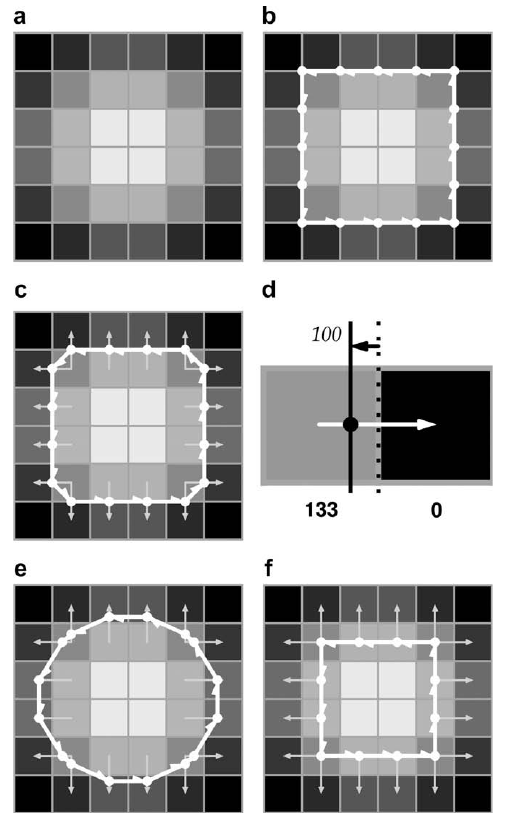
\includegraphics[width=.55\textwidth]{images/DICONEX_EX.png}
	\caption{Przykład działania algorytmu DICONEX na obrazie w skali szarości, o rozmiarach $6 \times 6$ \cite{Schlei2009}.}
	\label{fig:diconex_ex}
\end{figure}

\begin{figure}[ht]
	\centering
	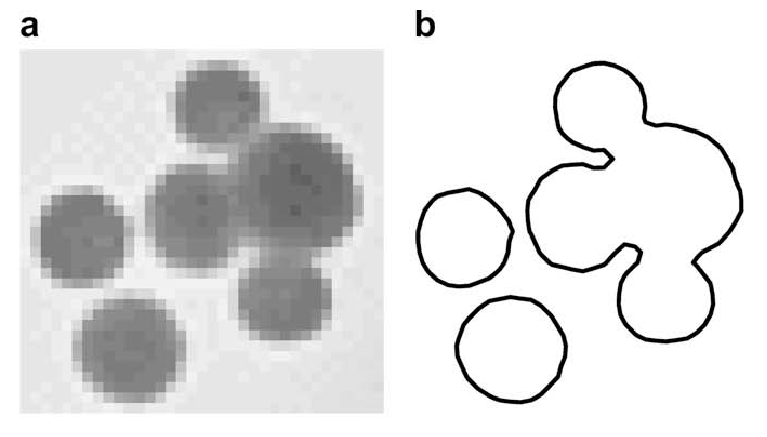
\includegraphics[width=.70\textwidth]{images/DICONEX_EX_RES.png}
	\caption{Wynik (b) działania algorytmu DICONEX na obrazie niewielkiej rozdzielczości (a) \cite{Schlei2009}.}
	\label{fig:diconex_ex_res}
\end{figure}

\label{dixonex_alg}
\subsubsection{Algorytm}

Na początku algorytmu wymagane jest wybranie jednej -- granicznej wartości jasności dla obrazu. W przykładzie z pracy \cite{Schlei2009}, dla obrazu, którego jasność piksli jest z zakresu $0 - 155$ została ona obrana na poziomie 100. Rysunek \ref{fig:diconex_ex}A przedstawia wejściowy obraz. W pierwszym kroku algorytmu, w obrazie wektorami konturowymi (ang. contour vector) otaczane są piksle o wartości jasności większej niż 100 -- czyli jasne piksle -- czego wynik przedstawiany jest na rysunku \ref{fig:diconex_ex}b. Warto zauważyć, że wspomniane wektory konturowe zawsze zwrócone są w taką stronę, że po lewej stronie mają otaczany obiekt -- czyli w tym wypadku piksle o jasności większej niż 100. Zgodnie z tym algorytmem zawsze znalezione wektory będą ze sobą połączone na zasadzie początek jednego wektora z końcem drugiego wektora i nie będzie pustych obszarów. Jako kolejny krok algorytmu, wszystkie stworzone wektory zamieniane są na inne wektory, o tej samej orientacji, ale ich punkty zaczepienia znajdują się w na środku wyznaczonego wcześniej wektora krawędziowego (konturowego), a kończą się w środku kolejnego wektora krawędziowego. Po zastosowaniu się do tego przekształcenia obraz otrzymany powinien wraz z krawędzią wyglądać tak jak na rysunku \ref{fig:diconex_ex}c. Dodatkowo na tym rysunku przedstawione są pewne wektory, które w cytowanej publikacji nazywane są wektorami zakresu (ang. range vector). Wektory te są umieszczone w obrazie w taki sposób, że łączą środki sąsiednich piksli i przechodzą przez każdy środek wektora konturowego a ich zwrot jest skierowany na zewnątrz otaczanego obszaru. Rysunek \ref{fig:diconex_ex}d przedstawia 2 piksle z obrazu, między którymi znajdował się środek wektora konturowego. W kolejnym kroku algorytmu punkt ten będzie przesunięty na wektorze zakresu w taki sposób, że obrana na samym początku wartość jasności (równa 100) będzie znajdować się na tym wektorze, gdy między środkowymi punktami piksli wartość ich jasności będzie liniowo interpolowana. Wynik takiego działania przedstawiony jest na rysunku \ref{fig:diconex_ex}e. Rysunek \ref{fig:diconex_ex}f przedstawia wynik transformacji tego poszerzonego konturu do konturu oznaczającego granicę szukanego obszaru. Jednak jak widać na przykładzie to przekształcenie jakby cofało wszystkie uogólnienia, zaokrąglenia i właściwie same przekształcenia, które zostały znalezione w obrazie \ref{fig:diconex_ex}c i \ref{fig:diconex_ex}e. Zdaniem autora najlepszy rezultat zaprezentowany jest na rysunku \ref{fig:diconex_ex}e.\\

O ile sam algorytm jest ciekawy, to został on tutaj zaprezentowany głównie z powodu na efekty, jakie można uzyskać w innych nietrywialnych obrazach, w a szczególności tych, niewielkich rozmiarów. Rysunek \ref{fig:diconex_ex_res} przedstawia wynik działania algorytmu na obrazie słabej rozdzielczości. Wyraźnie widać, że kontury odtworzone przez algorytm są wyraźne i gładkie, co jest niewątpliwą zaletą.\\

Z zastosowaniem tego algorytmu jest jednak podstawowy problem, który polega na konieczności obrania wartości granicznej dla jasności grup piksli w obrazie. Podobne problemy mają inne algorytmy odnajdujące krawędzie w obrazie. Można by się spierać, który jest lepszy, fakt jest jednak taki, że w oryginalnej postaci wymagają określania dodatkowych specyficznych parametrów.\\

Trochę inaczej można podejść do tego zagadnienia metodami zaczerpniętymi wprost z grafiki komputerowej -- filtrami. Dla obrazów binarnych (dwukolorowych) bardzo prosto jest określić okno filtru, który miałby odzyskać same krawędzie z obszarów przedstawionych w obrazie \cite{Tadeusiewicz}. Dla obrazów w skali szarości można posłużyć się bardziej zaawansowanymi filtrami, w tym na przykład filtrem Gabora, o którym dokładniej w części \ref{aGabor}.



